\chapter{Ist-Analyse der Suchoberfläche}

\section{Ausgangssituation}

\begin{figure}[htbp]
    \centering
    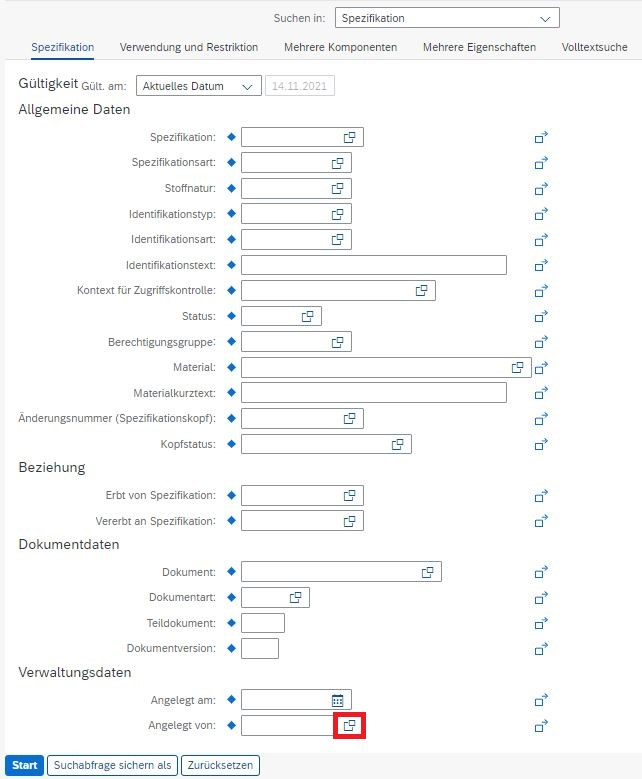
\includegraphics[width=0.9\textwidth]{img/LayoutRdavormitMarkierung.jpg}
    \caption[Bisherige Suchoberfläche der PLM-Spezifikation im Range View]{Bisherige Suchoberfläche der PLM-Spezifikation im Range View (Eigene Darstellung)}
    \label{fig:LayoutRdavor}
\end{figure}

Die Abbildung \ref{fig:LayoutRdavor} zeigt wie die \ac{plmwui}-Suche für das Objekt der Spezifikation vor der Umsetzung des Kundenwunsches aussieht. Es fällt auf, dass sämtliche Suchkriterien den Kategorien allgemeine Daten, Gültigkeit, Beziehung, Dokumentdaten und Verwaltungsdaten zugeordnet sind.

Die Felder der Suchkriterien mit dem in der Abbildung \ref{fig:LayoutRdavor} rot markierten Symbol rechts neben dem Eingabefeld verfügen über eine sogenannte F4-Hilfe. Beim Klicken auf das Icon oder drücken der F4-Taste, öffnet sich ein Selektionsbild, dass dem Benutzer eine Liste mit möglichen Werten für das jeweilige Suchkriterium vorschlägt. Um den gesucht Zielwert schneller zu finden, hat der Benutzer hier die Möglichkeit, die Selektionsliste mit weiteren Suchkriterien einzugrenzen. 


Der Web-Dynpro-Component für das Objekt der Spezifikation umfasst zwei Views, die beide bei Kunden im Einsatz sind. Der in der Abbildung \ref{fig:LayoutRdavor} gezeigte View, ist der sogenannte Range View. Dieser wurde nach dem ersten View, der im nachfolgenden Text als General View bezeichnet wird, entwickelt und bringt im Vergleich zu diesem neue Funktionalitäten mit sich. So lassen sich bei der F4-Hilfe des Range Views, wie der Name: Range View schon vermuten lässt, nicht nur Werte, sondern auch Wertebereiche für die Suchkriterien eintragen. Darüber hinaus können hier auch gezielt Ergebnisse über die F4-Hilfe ausgeschlossen werden.

Neben dem Merkmal unterscheiden sich die beiden Views ebenfalls im Aufbau des \ac{ui}s. Während sich die Suchoberfläche der General View aus Web-Dynpro Bausteinen, die in einer klaren Reihenfolge angeordnet sein müssen, zusammen setzt, wird das Web \ac{ui} der Range View vor allem über Quellcode und den dazugehörigen Methoden aufgebaut.


\section{Kundenanforderung}

Am 04.12.2020 wurde im Customer Connection Programm der Wunsch, die Suchoberfläche der Spezifikation um die Felder changed on und changed by zu erweitern, eingereicht. Die Suchkriterien sollen es dem Benutzer ermöglichen, nach dem Datum und der Person, die zuletzt eine Spezifikation bearbeitet hatte, zu filtern. Die neuen Suchmöglichkeiten sollen das Auffinden der gesuchten Spezifikation für den Endanwender noch effizienter gestalten und bieten somit einen kleinen, aber klar spürbaren Mehrwert für die Kunden.\autocite[Vgl.][]{ADSESPEC}

Als Referenzen für die Umsetzung wurden die \ac{plmwui}-Suchen der \ac{plm}-Objekte Rezepte, Materialstückliste und Dokumente genannt, bei denen die Funktionalität bereits erfolgreich umgesetzt wurde. Damit die Suchoberfläche der Spezifikation zu ihren Referenzen konsistent ist, sollen die Felder im Bereich der Verwaltungsdaten unter den Suchkriterien created on und created by platziert werden. Aufgrund der Tatsache, dass von acht Kunden, die für den Vorschlag gestimmt, nicht alle die SAP HANA als Datenbank benutzen, muss die Umsetzung auch mit der \acl{trex} kompatibel sein.\autocite[Vgl.][]{ADSESPEC}




